\chapter{血糖与糖尿病}\label{ch:g12:glucose-and-diabetes}

五升血液，每升含葡萄糖一克，合计五克，
约相当于一块方糖。仅大脑每小时就要消耗这些，白天
与夜间都不间断，且别无他物可用。然而，一天不进食的人，
或一口气吃下整块蛋糕者，都能使\omterm{def:g12:glucose-and-diabetes:glycaemia}{血糖}浓度
始终维持在同一数值上下零点几克每升之内——而
胰腺功能衰竭者则不然，
并伴随从口渴到昏迷的种种后果。本章讨论人体内受到最密切监测的数值、
维持其稳定的器官，
以及两种\omterm{def:g12:glucose-and-diabetes:diabetes}{糖尿病}中这些器官失效时会发生什么。

\section{受调节的恒定值}

\begin{definition}[血糖]\label{def:g12:glucose-and-diabetes:glycaemia}
称\emph{血糖}\index{血糖}为血浆中葡萄糖的浓度，
健康人餐前约为 \qty{1}{g/L}（\qty{5.5}{mmol/L}），
进食后一小时内升至 \qty{1.4}{g/L}，两小时内恢复，
禁食一整天后降至 \qty{0.7}{g/L}。
低于 \qty{0.5}{g/L} 时大脑功能失常（先是意识混乱，继而昏迷）；
高于 \qty{1.8}{g/L} 时葡萄糖会溢入尿液，长期
高于 \qty{1.3}{g/L} 会损伤血管和神经。血糖是一个
\emph{受调节的}量：由一个测量并纠正它的系统，使其数值保持
在某一设定值附近。
\end{definition}

\begin{proposition}[葡萄糖池及其通量]\label{prop:g12:glucose-and-diabetes:pool}
血液中的 \qty{5}{g} 葡萄糖构成一个“池”，大量葡萄糖流经该池。
\emph{输入}：餐后的小肠（一小时内可达
\qty{100}{g}），以及两餐之间的\emph{肝脏}，它从
其储存的\emph{\omterm{def:g10:exercise-and-energy:glycogen}{糖原}}（\qty{100}{g}，半天的用量）中释放葡萄糖，
并由\omterm{def:g10:chemistry-of-life:families}{氨基酸}和乳酸生成新的葡萄糖。
\emph{输出}：大脑（\qty{5}{g/h}，恒定），肌肉（从
数克到工作时的 \qty{100}{g/h} 不等）、其他组织，以及以
\omterm{def:g10:exercise-and-energy:glycogen}{糖原}形式储存于肝脏和肌肉中，或转化为脂肪。\qty{5}{g} 的池，
每小时以数十克的速度输入和输出，
之所以能保持稳定，全靠各流量逐分钟调节。
\end{proposition}
\admitted

\begin{omfigure}
\begin{tikzpicture}[font=\small, >=Stealth,
  b/.style={draw, rounded corners, align=center, minimum height=1.0cm}]
  \node[b, fill=omThm!15, text width=3.0cm, minimum height=1.6cm] (blood) at (0,0) {血糖 \\ \qty{5}{g}，约 \qty{1}{g/L}};
  \node[b, fill=omDef!12, text width=2.6cm] (gut) at (-4.5,1.6) {小肠 \\ （餐后）};
  \node[b, fill=omDef!12, text width=2.6cm] (liver) at (-4.5,-1.6) {肝脏：糖原 \\ 储存，新生葡萄糖};
  \node[b, fill=omMeth!15, text width=2.6cm] (brain) at (4.5,1.6) {大脑：\qty{5}{g/h}，\\ 仅利用葡萄糖};
  \node[b, fill=omMeth!15, text width=2.6cm] (muscle) at (4.5,0) {肌肉：利用，并 \\ 以糖原形式储存};
  \node[b, fill=omMeth!15, text width=2.6cm] (fat) at (4.5,-1.6) {脂肪组织：\\ 以脂肪形式储存};
  \draw[->, thick] (gut) -- (blood.west |- 0,0.5);
  \draw[<->, thick] (liver) -- node[below=1pt, font=\scriptsize, sloped] {双向} (blood.west |- 0,-0.5);
  \draw[->, thick] (blood.east |- 0,0.5) -- (brain);
  \draw[->, thick] (blood.east) -- (muscle);
  \draw[->, thick] (blood.east |- 0,-0.5) -- (fat);
\end{tikzpicture}

{\small 葡萄糖池。进餐和肝脏向其输入葡萄糖；大脑、
肌肉和脂肪组织则从中取出；只有肝脏能双向运行，
餐后储存，两餐之间释放。}
\end{omfigure}

\begin{example}[一天中的血糖]\label{ex:g12:glucose-and-diabetes:day}
8 点早餐：\omterm{def:g12:glucose-and-diabetes:glycaemia}{血糖}由 \num{0.9} 升至 \qty{1.3}{g/L}（9 点时），
10 点时回落至 \num{1.0}，多余的葡萄糖已转入肝脏
和肌肉的\omterm{def:g10:exercise-and-energy:glycogen}{糖原}。10 点至 13 点，肝脏释放\omterm{def:g10:exercise-and-energy:glycogen}{糖原}，\omterm{def:g12:glucose-and-diabetes:glycaemia}{血糖}
维持在 \num{0.9} 左右。17 点跑步时，一小时内有 \qty{60}{g} 葡萄糖流入
肌肉；肝脏为跟上需要，动用了一半的储存量，
\omterm{def:g12:glucose-and-diabetes:glycaemia}{血糖}降至 \num{0.8}。夜间，肝脏
以\omterm{def:g10:chemistry-of-life:families}{氨基酸}为原料生成新的葡萄糖，7 点时\omterm{def:g12:glucose-and-diabetes:glycaemia}{血糖}为 \qty{0.9}{g/L}。
一个仅五克的池中，共有三百克葡萄糖流过。
\end{example}

\section{胰腺维持平衡}

\begin{proposition}[胰岛分泌的两种激素]\label{prop:g12:glucose-and-diabetes:hormones}
胰腺中，在分泌消化酶的\omterm{def:g10:cells-common-unit:cell}{细胞}之间，
散布着约一百万个小\omterm{def:g10:cells-common-unit:cell}{细胞}团，即\emph{胰岛}\index{胰岛}。
\omterm{prop:g12:glucose-and-diabetes:hormones}{胰岛}\omterm{def:g10:cells-common-unit:cell}{细胞}测量流经的血液中的\omterm{def:g12:glucose-and-diabetes:glycaemia}{血糖}水平，
并向血液中分泌两种\omterm{def:g11:hormones-and-reproduction:hormone}{激素}：
\begin{itemize}
  \item \emph{胰岛素}\index{胰岛素}，由 $\beta$ \omterm{def:g10:cells-common-unit:cell}{细胞}分泌，当
        \omterm{def:g12:glucose-and-diabetes:glycaemia}{血糖}升高时：使肌肉和脂肪\omterm{def:g10:cells-common-unit:cell}{细胞}摄取葡萄糖，
        并使肝脏和肌肉将其以\omterm{def:g10:exercise-and-energy:glycogen}{糖原}形式储存；\omterm{def:g12:glucose-and-diabetes:glycaemia}{血糖}
        降低；
  \item \emph{胰高血糖素}\index{胰高血糖素}，由 $\alpha$ \omterm{def:g10:cells-common-unit:cell}{细胞}分泌，当
        \omterm{def:g12:glucose-and-diabetes:glycaemia}{血糖}降低时：促使肝脏分解\omterm{def:g10:exercise-and-energy:glycogen}{糖原}并释放
        葡萄糖；\omterm{def:g12:glucose-and-diabetes:glycaemia}{血糖}升高。
\end{itemize}
两者作用于相同的器官，方向相反；它们的
平衡由所测\omterm{def:g12:glucose-and-diabetes:glycaemia}{血糖}每隔几分钟重新设定，构成了
调节机制。\omterm{prop:g12:glucose-and-diabetes:hormones}{胰岛素}是唯一能降低\omterm{def:g12:glucose-and-diabetes:glycaemia}{血糖}的\omterm{def:g11:hormones-and-reproduction:hormone}{激素}；
多种\omterm{def:g11:hormones-and-reproduction:hormone}{激素}能使其升高。
\end{proposition}
\begin{proof}[证据]
切除狗的胰腺（1889 年）后，一天之内它便患上\omterm{def:g12:glucose-and-diabetes:diabetes}{糖尿病}：
其\omterm{def:g12:glucose-and-diabetes:glycaemia}{血糖}升至三倍，尿液中出现葡萄糖；结扎
输送消化酶的导管则不会产生此效应，故该效应并非源于消化作用。
注射\omterm{prop:g12:glucose-and-diabetes:hormones}{胰岛}提取物（1921 年）可降低\omterm{def:g12:glucose-and-diabetes:diabetes}{糖尿病}狗的
及\omterm{def:g12:glucose-and-diabetes:diabetes}{糖尿病}儿童的\omterm{def:g12:glucose-and-diabetes:glycaemia}{血糖}，数小时之内即见效；
有效成分\omterm{prop:g12:glucose-and-diabetes:hormones}{胰岛素}于同年被提纯。离体\omterm{prop:g12:glucose-and-diabetes:hormones}{胰岛}置于培养皿中时，培养基葡萄糖浓度
升高时分泌\omterm{prop:g12:glucose-and-diabetes:hormones}{胰岛素}，降低时分泌\omterm{prop:g12:glucose-and-diabetes:hormones}{胰高血糖素}。注射\omterm{prop:g12:glucose-and-diabetes:hormones}{胰高血糖素}
可在数分钟内升高禁食者的\omterm{def:g12:glucose-and-diabetes:glycaemia}{血糖}，且仅当肝脏
储存有\omterm{def:g10:exercise-and-energy:glycogen}{糖
原}时才有效。
\end{proof}

\begin{omfigure}
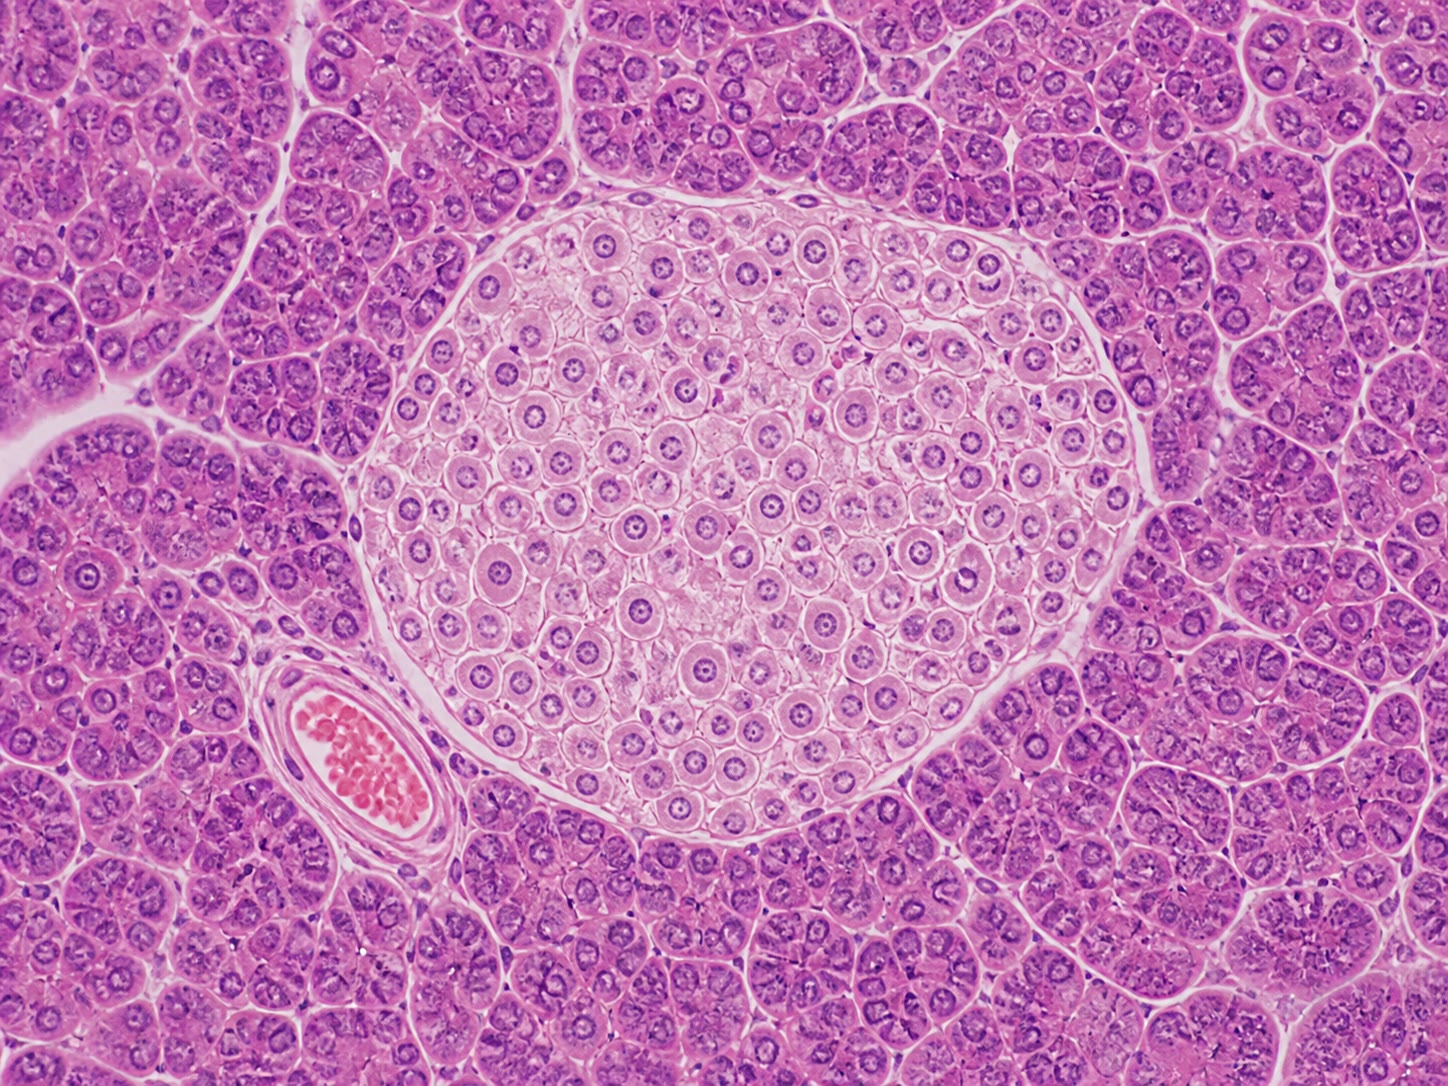
\includegraphics[width=0.56\linewidth]{images/book2/ai/g12-glucose-pancreas-islet.jpg}

{\small 胰腺切片：一个颜色较浅的\omterm{prop:g12:glucose-and-diabetes:hormones}{胰岛}，夹在
颜色较深的分泌消化酶的\omterm{def:g10:cells-common-unit:cell}{细胞}团之间。\omterm{prop:g12:glucose-and-diabetes:hormones}{胰岛}\omterm{def:g10:cells-common-unit:cell}{细胞}读取血液中的
葡萄糖，并以\omterm{prop:g12:glucose-and-diabetes:hormones}{胰岛素}或\omterm{prop:g12:glucose-and-diabetes:hormones}{胰高血糖素}作出应答；器官的其余部分
分泌消化液。}
\end{omfigure}

\begin{omfigure}
\begin{tikzpicture}[font=\small, >=Stealth,
  b/.style={draw, rounded corners, align=center, minimum height=1.0cm}]
  \node[b, fill=omThm!15, text width=3.2cm, minimum height=1.4cm] (gly) at (0,0) {血糖 \\ （设定点 \qty{1}{g/L}）};
  \node[b, fill=omProp!15, text width=2.8cm] (beta) at (-4.6,2.0) {$\beta$ 细胞：胰岛素};
  \node[b, fill=omProp!15, text width=2.8cm] (alpha) at (-4.6,-2.0) {$\alpha$ 细胞：胰高血糖素};
  \node[b, fill=omMeth!15, text width=3.4cm] (store) at (5.6,2.2) {肝脏、肌肉、脂肪：\\ 摄取并储存葡萄糖};
  \node[b, fill=omMeth!15, text width=3.4cm] (rel) at (5.6,-2.2) {肝脏：分解糖原 \\ 释放葡萄糖};
  \draw[->, thick] (gly.west |- 0,0.4) -- node[above, sloped, font=\scriptsize] {检测到上升} (beta.east);
  \draw[->, thick] (gly.west |- 0,-0.4) -- node[below, sloped, font=\scriptsize] {检测到下降} (alpha.east);
  \draw[->, thick, omProp] (beta.north) -- ++(0,0.6) -| (store.north);
  \draw[->, thick, omProp] (alpha.south) -- ++(0,-0.6) -| (rel.south);
  \draw[->, thick, omThm] (store.west) -- node[above, sloped, font=\scriptsize, align=center] {血糖 \\ 下降 $(-)$} (gly.east |- 0,0.4);
  \draw[->, thick, omThm] (rel.west) -- node[below, sloped, font=\scriptsize, align=center] {血糖 \\ 上升 $(+)$} (gly.east |- 0,-0.4);
  \node[font=\scriptsize, anchor=south] at (0,3.3) {胰岛素};
  \node[font=\scriptsize, anchor=north] at (0,-3.3) {胰高血糖素};
\end{tikzpicture}

{\small \omterm{def:g12:glucose-and-diabetes:glycaemia}{血糖}的调节。\omterm{def:g12:glucose-and-diabetes:glycaemia}{血糖}升高时触发\omterm{prop:g12:glucose-and-diabetes:hormones}{胰岛素}分泌，\omterm{prop:g12:glucose-and-diabetes:hormones}{胰岛素}
促使组织摄取并储存葡萄糖，使\omterm{def:g12:glucose-and-diabetes:glycaemia}{血糖}降低；\omterm{def:g12:glucose-and-diabetes:glycaemia}{血糖}下降时
触发\omterm{prop:g12:glucose-and-diabetes:hormones}{胰高血糖素}分泌，\omterm{prop:g12:glucose-and-diabetes:hormones}{胰高血糖素}促使肝脏释放葡萄糖，使\omterm{def:g12:glucose-and-diabetes:glycaemia}{血糖}回升。
每种\omterm{def:g11:hormones-and-reproduction:hormone}{激素}的作用都会消除引发它分泌的信号：两个
围绕同一设定点的负\omterm{def:g11:hormones-and-reproduction:hormone}{反馈}回路。}
\end{omfigure}

\begin{example}[回路的运作]\label{ex:g12:glucose-and-diabetes:loop}
进餐后\omterm{def:g12:glucose-and-diabetes:glycaemia}{血糖}升高；几分钟内 $\beta$ \omterm{def:g10:cells-common-unit:cell}{细胞}
分泌\omterm{prop:g12:glucose-and-diabetes:hormones}{胰岛素}，肌肉和脂肪\omterm{def:g10:cells-common-unit:cell}{细胞}打开葡萄糖转运蛋白，肝脏
转而合成\omterm{def:g10:exercise-and-energy:glycogen}{糖原}，\omterm{def:g12:glucose-and-diabetes:glycaemia}{血糖}回落，
\omterm{prop:g12:glucose-and-diabetes:hormones}{胰岛素}分泌也随之减少。
两餐之间\omterm{def:g12:glucose-and-diabetes:glycaemia}{血糖}缓慢下降，由\omterm{prop:g12:glucose-and-diabetes:hormones}{胰高血糖素}应对，\omterm{def:g10:exercise-and-energy:glycogen}{糖原}被分解，
\omterm{def:g12:glucose-and-diabetes:glycaemia}{血糖}得以维持稳定。两种\omterm{def:g11:hormones-and-reproduction:hormone}{激素}从不缺席，变化的是它们的比例，
\omterm{def:g12:glucose-and-diabetes:glycaemia}{血糖}则随之在狭窄的范围内波动。
\end{example}

\section{反馈回路失效：糖尿病}

\begin{definition}[糖尿病]\label{def:g12:glucose-and-diabetes:diabetes}
\emph{糖尿病}\index{糖尿病}是一种慢性的\omterm{def:g12:glucose-and-diabetes:glycaemia}{血糖}过高：
空腹\omterm{def:g12:glucose-and-diabetes:glycaemia}{血糖}高于 \qty{1.26}{g/L}，或标准葡萄糖负荷后两小时高于 \qty{2}{g/L}。
其早期症状由\omterm{def:g12:glucose-and-diabetes:glycaemia}{血糖}过高引起：尿液中出现葡萄糖，
葡萄糖会带走水分，使尿量增多、口渴；
\omterm{def:g10:cells-common-unit:cell}{细胞}无法利用周围的葡萄糖时，体重下降。其晚期损伤——
包括眼和肾的小血管、神经以及动脉的病变——
是多年葡萄糖与\omterm{def:g11:gene-expression:protein}{蛋白质}反应的结果。
两种疾病共用这一名称。
\end{definition}

\begin{proposition}[1 型与 2 型]\label{prop:g12:glucose-and-diabetes:types}
\begin{itemize}
  \item \emph{1 型\omterm{def:g12:glucose-and-diabetes:diabetes}{糖尿病}}（约占病例的 10\%）是患者
        自身免疫系统对 $\beta$ \omterm{def:g10:cells-common-unit:cell}{细胞}的破坏，
        多发于儿童或青少年，体内缺乏\omterm{prop:g12:glucose-and-diabetes:hormones}{胰岛素}。\omterm{def:g12:glucose-and-diabetes:glycaemia}{血糖}
        不受控制地升高，因缺少可利用的葡萄糖，脂肪被分解供能，
        其酸性产物不断积累；不注射\omterm{prop:g12:glucose-and-diabetes:hormones}{胰岛素}，
        数月内即可致死。治疗方法是终身注射\omterm{prop:g12:glucose-and-diabetes:hormones}{胰岛素}，
        每天数次，剂量依据进餐情况与
        实测\omterm{def:g12:glucose-and-diabetes:glycaemia}{血糖}确定。
  \item \emph{2 型\omterm{def:g12:glucose-and-diabetes:diabetes}{糖尿病}}（约占 90\%）多发于成人，
        且多见于超重、缺乏运动者：组织对\omterm{prop:g12:glucose-and-diabetes:hormones}{胰岛素}的反应
        逐渐减弱（\emph{\omterm{prop:g12:glucose-and-diabetes:hormones}{胰岛素}抵抗}），$\beta$ \omterm{def:g10:cells-common-unit:cell}{细胞}
        代偿性地分泌更多\omterm{prop:g12:glucose-and-diabetes:hormones}{胰岛素}，多年后逐渐耗竭。
        \omterm{prop:g12:glucose-and-diabetes:hormones}{胰岛素}并非缺失，而是不足。其
        易感性部分受遗传影响
        （见\cref{ch:g11:genes-and-disease}）；诱因则是生活方式，
        因此首选治疗是改变它——减重与运动——
        然后才是药物，晚期才用\omterm{prop:g12:glucose-and-diabetes:hormones}{胰岛素}。
\end{itemize}
\end{proposition}
\begin{proof}[证据]
1 型患者在症状出现前数年，体内即已产生针对自身\omterm{prop:g12:glucose-and-diabetes:hormones}{胰岛}\omterm{def:g10:cells-common-unit:cell}{细胞}的抗体，
确诊时其\omterm{prop:g12:glucose-and-diabetes:hormones}{胰岛}几乎已无
$\beta$ \omterm{def:g10:cells-common-unit:cell}{细胞}，并有白\omterm{def:g10:cells-common-unit:cell}{细胞}浸润；其血液中\omterm{prop:g12:glucose-and-diabetes:hormones}{胰岛素}
检测不到，注射\omterm{prop:g12:glucose-and-diabetes:hormones}{胰岛素}后立即起效。2 型患者
确诊时\omterm{prop:g12:glucose-and-diabetes:hormones}{胰岛素}水平正常或偏高；其肌肉和脂肪\omterm{def:g10:cells-common-unit:cell}{细胞}
在同等\omterm{prop:g12:glucose-and-diabetes:hormones}{胰岛素}剂量下，摄取葡萄糖的能力比健康人弱；
同卵双胞胎中有 70\% 的病例共患此病，
仅靠减重或步行计划，就能使许多
早期病例的\omterm{def:g12:glucose-and-diabetes:glycaemia}{血糖}恢复正常。
\end{proof}

\begin{omfigure}
\begin{tikzpicture}
\begin{axis}[
  width=0.88\linewidth, height=5.8cm,
  axis x line=bottom, axis y line=left,
  xmin=0, xmax=180, ymin=0, ymax=3,
  xlabel={饮用 \qty{75}{g} 葡萄糖后的时间（分钟）}, ylabel={血糖（g/L）},
  xlabel style={font=\small, at={(axis description cs:0.5,-0.12)}, anchor=north},
  ylabel style={font=\small},
  tick label style={font=\small}, xtick={0,30,60,90,120,150,180}, ytick={0,1,2,3},
  legend style={at={(0.5,-0.3)}, anchor=north, legend columns=3, font=\small, draw=none},
  clip=false,
]
\addplot[thick, omMeth, smooth] coordinates {(0,0.9) (30,1.4) (60,1.3) (90,1.1) (120,0.95) (150,0.9) (180,0.9)};
\addplot[thick, omProp, smooth] coordinates {(0,1.1) (30,1.7) (60,1.9) (90,1.85) (120,1.7) (150,1.5) (180,1.35)};
\addplot[thick, omThm, smooth] coordinates {(0,1.6) (30,2.3) (60,2.7) (90,2.8) (120,2.7) (150,2.6) (180,2.5)};
\draw[dashed, gray] (axis cs:0,2) -- (axis cs:180,2);
\node[font=\scriptsize, gray, anchor=south east] at (axis cs:180,2.02) {120 分钟时的阈值};
\legend{健康人, 糖耐量受损, 2 型糖尿病}
\end{axis}
\end{tikzpicture}

{\small 葡萄糖耐量试验：服用标准葡萄糖饮剂后的\omterm{def:g12:glucose-and-diabetes:glycaemia}{血糖}，
即 \qty{75}{g} 葡萄糖。健康人在两小时内\omterm{def:g12:glucose-and-diabetes:glycaemia}{血糖}
回落至接近 \qty{1}{g/L}；\omterm{def:g12:glucose-and-diabetes:diabetes}{糖尿病}患者起始\omterm{def:g12:glucose-and-diabetes:glycaemia}{血糖}即较高，升至 \qty{2}{g/L} 以上并
持续在此水平。中间曲线为预警阶段，通常
可逆。}
\end{omfigure}

\begin{example}[1 型糖尿病患者一天的管理]\label{ex:g12:glucose-and-diabetes:type1}
一名 1 型\omterm{def:g12:glucose-and-diabetes:diabetes}{糖尿病}少女每餐前测定\omterm{def:g12:glucose-and-diabetes:glycaemia}{血糖}，
用一滴血测定，数出餐盘上的碳水化合物，并注射
一剂速效\omterm{prop:g12:glucose-and-diabetes:hormones}{胰岛素}，剂量与之成正比，约每
\qty{10}{g} 注射 1 单位；另每日一次长效\omterm{prop:g12:glucose-and-diabetes:hormones}{胰岛素}维持基础。
\omterm{prop:g12:glucose-and-diabetes:hormones}{胰岛素}过量或漏餐时，\omterm{def:g12:glucose-and-diabetes:glycaemia}{血糖}会降至
\qty{0.6}{g/L} 以下：出汗、颤抖、意识模糊，
数分钟内补充糖分即可纠正。\omterm{prop:g12:glucose-and-diabetes:hormones}{胰岛素}不足时，
\omterm{def:g12:glucose-and-diabetes:glycaemia}{血糖}持续高于 \qty{2}{g/L}，伴有口渴、乏力，血管则悄然受损。她
正以手工方式做 $\beta$ \omterm{def:g10:cells-common-unit:cell}{细胞}借\omterm{def:g11:hormones-and-reproduction:hormone}{反馈}所做的事。
\end{example}

\begin{omfigure}
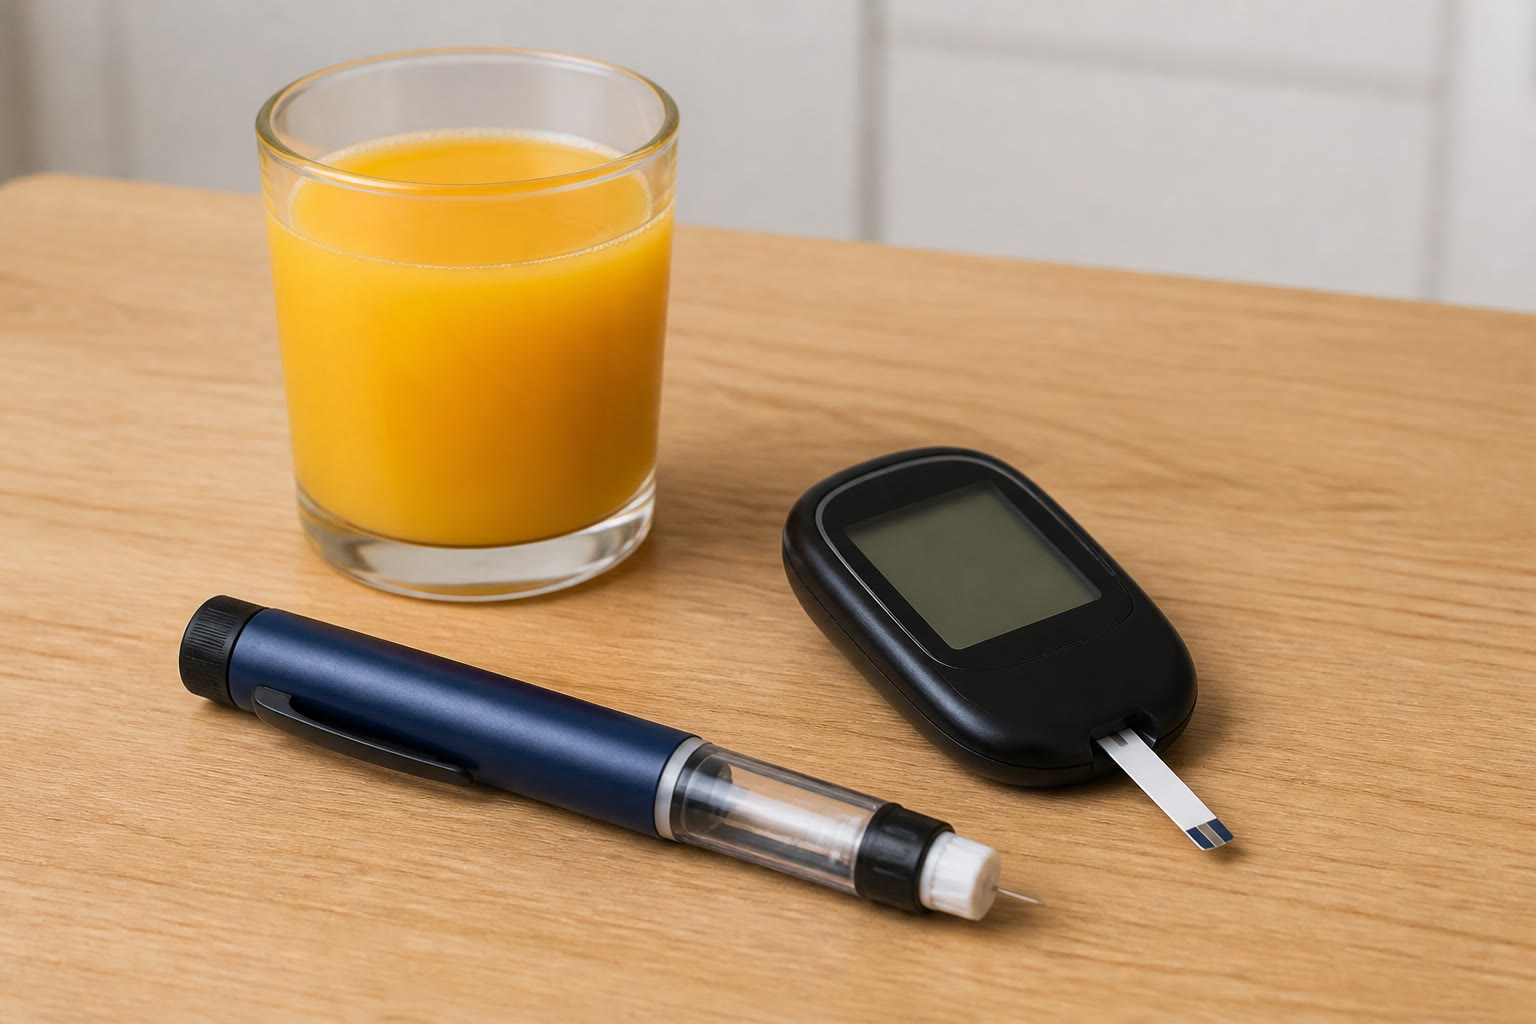
\includegraphics[width=0.56\linewidth]{images/book2/ai/g12-glucose-meter-pen.jpg}

{\small 1 型\omterm{def:g12:glucose-and-diabetes:diabetes}{糖尿病}患者的器具：一台仪器可由一滴血读出
\omterm{def:g12:glucose-and-diabetes:glycaemia}{血糖}，另有一支笔可注射定量的\omterm{prop:g12:glucose-and-diabetes:hormones}{胰岛素}。
\omterm{prop:g12:glucose-and-diabetes:hormones}{胰岛}的调节环路，每日需人工操作数次。}
\end{omfigure}

\begin{method}[读取血糖记录]\label{met:g12:glucose-and-diabetes:read}
\begin{enumerate}
  \item 找出设定点与正常范围：空腹 \qtyrange{0.7}{1.1}{g/L}，
        餐后低于 \num{1.4}；葡萄糖负荷两小时后
        低于 \num{1.4}（健康），\qtyrange{1.4}{2}{}（糖耐量受损），
        高于 \qty{2}{g/L}（\omterm{def:g12:glucose-and-diabetes:diabetes}{糖尿病}）。
  \item 对每次升高，询问葡萄糖从何而来（进餐、肝脏），
        应由何种途径移出（\omterm{prop:g12:glucose-and-diabetes:hormones}{胰岛素}的作用靶点）；对每次下降，询问
        何者移出了葡萄糖（脑、肌肉），应由何者使其回升
        （\omterm{prop:g12:glucose-and-diabetes:hormones}{胰高血糖素}、肝脏）。
  \item 结合葡萄糖读取\omterm{def:g11:hormones-and-reproduction:hormone}{激素}：\omterm{prop:g12:glucose-and-diabetes:hormones}{胰岛素}应随\omterm{def:g12:glucose-and-diabetes:glycaemia}{血糖}升高而上升，
        \omterm{prop:g12:glucose-and-diabetes:hormones}{胰高血糖素}则应下降；无\omterm{prop:g12:glucose-and-diabetes:hormones}{胰岛素}提示 1 型\omterm{def:g12:glucose-and-diabetes:diabetes}{糖尿病}，
        \omterm{prop:g12:glucose-and-diabetes:hormones}{胰岛素}高而\omterm{def:g12:glucose-and-diabetes:glycaemia}{血糖}也高，提示存在\omterm{prop:g12:glucose-and-diabetes:hormones}{胰岛素}抵抗。
  \item 必要时换算单位：\qty{1}{g/L} 葡萄糖相当于
        \qty{5.55}{mmol/L}。
\end{enumerate}
\end{method}

\begin{remark}[调节的一个模型]\label{rem:g12:glucose-and-diabetes:model}
感受器、设定点、两个相反作用的效应器与负\omterm{def:g11:hormones-and-reproduction:hormone}{反馈}：
\omterm{def:g12:glucose-and-diabetes:glycaemia}{血糖}的调控与睾酮的调控采用同一设计，
在\cref{ch:g11:hormones-and-reproduction}中；体内多数恒定量的设计亦然，
——如体温、水分、血压与酸碱度。
\omterm{def:g12:glucose-and-diabetes:diabetes}{糖尿病}即为调节环路被破坏时，恒定量呈现的样子：
数值仍会随输入变化，却无力使其回归。
读懂本章的曲线，就是在练习读懂任何一条
此类曲线。
\end{remark}

\section{练习}

\begin{exercise}[$\star$]\label{exo:g12:glucose-and-diabetes:1}
求空腹正常\omterm{def:g12:glucose-and-diabetes:glycaemia}{血糖}值，分别用 \unit{g/L} 和 \unit{mmol/L} 表示，
以及两个危险阈值。
\end{exercise}

\begin{exercise}[$\star$]\label{exo:g12:glucose-and-diabetes:2}
写出\omterm{prop:g12:glucose-and-diabetes:hormones}{胰岛}产生的两种\omterm{def:g11:hormones-and-reproduction:hormone}{激素}、产生它们的\omterm{def:g10:cells-common-unit:cell}{细胞}以及
各自对\omterm{def:g12:glucose-and-diabetes:glycaemia}{血糖}的作用。
\end{exercise}

\begin{exercise}[$\star$]\label{exo:g12:glucose-and-diabetes:3}
哪一器官既能储存又能释放葡萄糖？
它以何种形式储存？
\end{exercise}

\begin{exercise}[$\star$]\label{exo:g12:glucose-and-diabetes:4}
分别用一句话说明 1 型与 2 型\omterm{def:g12:glucose-and-diabetes:diabetes}{糖尿病}的
本质区别。
\end{exercise}

\begin{exercise}[$\star$]\label{exo:g12:glucose-and-diabetes:5}
由葡萄糖耐量试验图读出 120 分钟时三条曲线的数值，
并对每条曲线进行分类。
\end{exercise}

\begin{exercise}[$\star\star$]\label{exo:g12:glucose-and-diabetes:6}
脑每小时消耗 \qty{5}{g} 葡萄糖，而血液中仅含
\qty{5}{g}。试解释为何进餐一小时后人不会失去意识，
并指出起作用的器官与\omterm{def:g11:hormones-and-reproduction:hormone}{激素}。
\end{exercise}

\begin{exercise}[$\star\star$]\label{exo:g12:glucose-and-diabetes:7}
试解释为何切除胰腺会导致\omterm{def:g12:glucose-and-diabetes:diabetes}{糖尿病}，而结扎其导管
则不会，这说明\omterm{prop:g12:glucose-and-diabetes:hormones}{胰岛素}产生于何处、如何
到达作用部位。
\end{exercise}

\begin{exercise}[$\star\star$]\label{exo:g12:glucose-and-diabetes:8}
一名空腹者注射\omterm{prop:g12:glucose-and-diabetes:hormones}{胰高血糖素}，\omterm{def:g12:glucose-and-diabetes:glycaemia}{血糖}
在 20 分钟内升高 \qty{0.4}{g/L}。同样的注射在禁食三天后
则毫无作用。请解释。
\end{exercise}

\begin{exercise}[$\star\star$]\label{exo:g12:glucose-and-diabetes:9}
\omterm{def:g12:glucose-and-diabetes:diabetes}{糖尿病}患者为何排尿量多且感到口渴？
\end{exercise}

\begin{exercise}[$\star\star$]\label{exo:g12:glucose-and-diabetes:10}
一名 1 型患者注射了平常剂量的\omterm{prop:g12:glucose-and-diabetes:hormones}{胰岛素}，随后
不进午餐。试预测其后两小时会发生什么，并说明原因。
\end{exercise}

\begin{exercise}[$\star\star$]\label{exo:g12:glucose-and-diabetes:11}
试解释为何运动能降低 2 型\omterm{def:g12:glucose-and-diabetes:diabetes}{糖尿病}患者的\omterm{def:g12:glucose-and-diabetes:glycaemia}{血糖}，
即使\omterm{prop:g12:glucose-and-diabetes:hormones}{胰岛素}水平没有任何变化，并结合\cref{ch:g10:sport-and-health}加以说明。
\end{exercise}

\begin{exercise}[$\star\star\star$]\label{exo:g12:glucose-and-diabetes:12}
两名患者的空腹\omterm{def:g12:glucose-and-diabetes:glycaemia}{血糖}均为 \qty{2}{g/L}。其中一人
检测不到\omterm{prop:g12:glucose-and-diabetes:hormones}{胰岛素}，另一人的\omterm{prop:g12:glucose-and-diabetes:hormones}{胰岛素}为正常值的三倍。
请分别作出诊断，并说明每位患者的\omterm{prop:g12:glucose-and-diabetes:hormones}{胰岛}正在做什么。
\end{exercise}

\begin{exercise}[$\star\star\star$]\label{exo:g12:glucose-and-diabetes:13}
  画出或描述餐后三小时内
健康人、未经治疗的 1 型患者及 2 型患者的\omterm{def:g12:glucose-and-diabetes:glycaemia}{血糖}与\omterm{prop:g12:glucose-and-diabetes:hormones}{胰岛素}曲线，
并解释每项差异。
\end{exercise}

\begin{exercise}[$\star\star\star$]\label{exo:g12:glucose-and-diabetes:14}
一餐含有 \qty{80}{g} 碳水化合物。若其全部
一次性进入血液，\omterm{def:g12:glucose-and-diabetes:glycaemia}{血糖}将升至多少？解释为何实际上从未如此，
并列出前两小时内葡萄糖的去向。
\end{exercise}

\begin{exercise}[$\star\star\star$]\label{exo:g12:glucose-and-diabetes:15}
比较\omterm{def:g12:glucose-and-diabetes:glycaemia}{血糖}的调节与
\cref{ch:g11:hormones-and-reproduction}中的睾酮调节，
从感受器、设定点、效应器和\omterm{def:g11:hormones-and-reproduction:hormone}{反馈}的符号等方面进行比较。
两种\omterm{def:g11:hormones-and-reproduction:hormone}{激素}相互拮抗，这种安排有何特殊之处？
\end{exercise}

\section{问题：五克糖}

\begin{problem}[{周末问题——一日内血糖的核算：
血糖池及其流量、耐量试验的判读，
胰岛素剂量的计算，以及需要人工代替的
调节回路}]
\label{pb:g12:glucose-and-diabetes:1}
设血液体积为 \qty{5}{L}，脑的葡萄糖消耗速率为
\qty{5}{g/h}，肝\omterm{def:g10:exercise-and-energy:glycogen}{糖原}储量为 \qty{100}{g}，
肌\omterm{def:g10:exercise-and-energy:glycogen}{糖原}为 \qty{400}{g}。一单位速效\omterm{prop:g12:glucose-and-diabetes:hormones}{胰岛素}可处理
约 \qty{10}{g} 碳水化合物。

\medskip
\noindent\textbf{第一部分——\omterm{def:g12:glucose-and-diabetes:glycaemia}{血糖}池。}
\begin{enumerate}
  \item 计算血液中葡萄糖浓度为 \qty{1}{g/L} 时的质量，
        并以 \unit{mmol/L} 表示同一浓度（葡萄糖
        摩尔质量为 \qty{180}{g/mol}）。
  \item 若无任何补充，血液中的葡萄糖仅供脑使用，
        能维持多长时间？
  \item 两餐之间由肝脏补充。肝\omterm{def:g10:exercise-and-energy:glycogen}{糖原}可供脑使用
        多长时间？此后会怎样？
  \item 肌\omterm{def:g10:exercise-and-energy:glycogen}{糖原}量是肝\omterm{def:g10:exercise-and-energy:glycogen}{糖原}的四倍，但肌肉不能
        将葡萄糖释放入血。解释肌\omterm{def:g10:exercise-and-energy:glycogen}{糖原}为何不能
        帮助脑，并说明它的用途。
  \item 一餐在一小时内提供 \qty{60}{g} 葡萄糖。若
        不作清除，\omterm{def:g12:glucose-and-diabetes:glycaemia}{血糖}将升至多少？实际上由什么清除它，
        它又去向何处？
\end{enumerate}

\medskip
\noindent\textbf{第二部分——耐量试验。}
患者口服 \qty{75}{g} 葡萄糖，测得的\omterm{def:g12:glucose-and-diabetes:glycaemia}{血糖}与
\omterm{prop:g12:glucose-and-diabetes:hormones}{胰岛素}数值如下：

\begin{center}
\begin{tabular}{lcccccc}
分钟 & 0 & 30 & 60 & 90 & 120 & 180 \\ \hline
\omterm{def:g12:glucose-and-diabetes:glycaemia}{血糖}（g/L） & 1.15 & 1.8 & 2.05 & 2.0 & 1.85 & 1.6 \\
\omterm{prop:g12:glucose-and-diabetes:hormones}{胰岛素}（占健康峰值的 \%） & 90 & 140 & 180 & 200 & 190 & 160 \\
\end{tabular}
\end{center}
\begin{enumerate}[resume]
  \item 依据
        \cref{met:g12:glucose-and-diabetes:read}中的阈值对患者分类。
  \item \omterm{prop:g12:glucose-and-diabetes:hormones}{胰岛素}是否缺乏？若不缺乏，那么是什么出了故障？
  \item 写出疾病名称，并列出你预期患者病史中的
        两项特征。
  \item 若是未经治疗的 1 型患者，
        同一张表格将呈现怎样的结果？
  \item 首选治疗是什么？它
        通过何种机制起作用？
\end{enumerate}

\medskip
\noindent\textbf{第三部分——人工运行调节回路。}
1 型患者晚餐前的\omterm{def:g12:glucose-and-diabetes:glycaemia}{血糖}为 \qty{1.0}{g/L}；该餐
含碳水化合物 \qty{90}{g}。
\begin{enumerate}[resume]
  \item 计算该餐所需的速效\omterm{prop:g12:glucose-and-diabetes:hormones}{胰岛素}剂量。
  \item 她注射了\omterm{prop:g12:glucose-and-diabetes:hormones}{胰岛素}，但只吃了半餐。估计\omterm{def:g12:glucose-and-diabetes:glycaemia}{血糖}可能
        下降多少，并说出相应的症状与应对措施。
  \item 她不注射\omterm{prop:g12:glucose-and-diabetes:hormones}{胰岛素}，并吃下整餐。估算
        若 \qty{90}{g} 全部进入 \qty{5}{L} 的血液池时的\omterm{def:g12:glucose-and-diabetes:glycaemia}{血糖}值，
        并说明\omterm{def:g12:glucose-and-diabetes:glycaemia}{血糖}高于 \qty{1.8}{g/L} 时肾脏会做什么。
  \item 她夜间不进食，为何仍必须
        注射长效\omterm{prop:g12:glucose-and-diabetes:hormones}{胰岛素}？
  \item 解释\omterm{def:g12:glucose-and-diabetes:glycaemia}{血糖}仪与注射笔在何种意义上替代了
        $\beta$ \omterm{def:g10:cells-common-unit:cell}{细胞}，并说明它们无法替代什么。
\end{enumerate}

\medskip
\noindent\textbf{第四部分——调节回路的推理。}
\begin{enumerate}[resume]
  \item 某种药物可刺激 $\beta$ \omterm{def:g10:cells-common-unit:cell}{细胞}分泌更多\omterm{prop:g12:glucose-and-diabetes:hormones}{胰岛素}。
        该药物可对哪一类\omterm{def:g12:glucose-and-diabetes:diabetes}{糖尿病}起效，并说明
        为何对另一类无效？
  \item 一名 2 型患者减重 \qty{10}{kg}，每天步行
        一小时；六个月后耐量试验结果恢复正常。解释
        调节回路的哪一部分得到了修复。
  \item 解释健康人的\omterm{prop:g12:glucose-and-diabetes:hormones}{胰岛素}与\omterm{prop:g12:glucose-and-diabetes:hormones}{胰高血糖素}为何从不会
        同时处于高水平，并说明体外培养的\omterm{prop:g12:glucose-and-diabetes:hormones}{胰岛}在
        培养基葡萄糖浓度设为 \qty{1}{g/L} 时会有何反应。
  \item \omterm{prop:g12:glucose-and-diabetes:hormones}{胰高血糖素}、\omterm{prop:g10:heart-lungs-effort:control}{肾上腺素}、皮质醇与生长\omterm{def:g11:hormones-and-reproduction:hormone}{激素}均可升高
        \omterm{def:g12:glucose-and-diabetes:glycaemia}{血糖}，只有\omterm{prop:g12:glucose-and-diabetes:hormones}{胰岛素}能降低\omterm{def:g12:glucose-and-diabetes:glycaemia}{血糖}。试推测机体为何
        对低\omterm{def:g12:glucose-and-diabetes:glycaemia}{血糖}设有多重保障，而对高\omterm{def:g12:glucose-and-diabetes:glycaemia}{血糖}的保障
        只有一重。
  \item 给出结果：血液中的葡萄糖量、肝脏可维持的
        小时数、第二部分的诊断，以及第三部分的
        剂量。
\end{enumerate}
\end{problem}
